\begin{frame}{From Scalars to Vectors}
    \framesubtitle{Efficient Implementation}
    \begin{itemize}
        \item While the computational graph concept works for single values (scalars), neural networks are implemented using \bhighlight{vectors and matrices} for efficiency.
        \item Instead of calculating gradients one by one, we can process an entire layer or even a mini-batch of data with a few matrix operations.
    \end{itemize}
\end{frame}

\begin{frame}{From Scalars to Vectors}
    \framesubtitle{The Jacobian Matrix}
    \begin{columns}[c]
        \begin{column}{0.5\linewidth}
            \begin{itemize}
                \item The derivative of a vector function with respect to a vector input is a matrix of all possible partial derivatives, called the \bhighlight{Jacobian}.
                \item For a layer's activation $a = f(z)$, the Jacobian $\frac{\partial a}{\partial z}$ tells us how a small change in each input element $z_i$ affects each output element $a_j$.
            \end{itemize}
        \end{column}
        \begin{column}{0.5\linewidth}
            \begin{figure}
                \centering
                % Source: MLP & Back-prop.pdf, Page: 73
                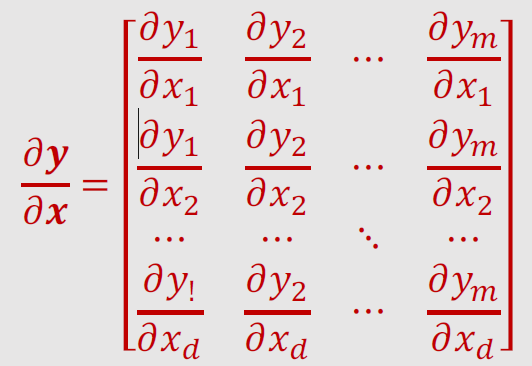
\includegraphics[width=0.8\linewidth]{images/jacobian_matrix.png}
                \caption{Structure of a Jacobian matrix.}
            \end{figure}
        \end{column}
    \end{columns}
\end{frame}

\begin{frame}{From Scalars to Vectors}
    \framesubtitle{Vectorized Forward \& Backward Pass}
    \begin{itemize}
        \item \textbf{Forward Pass:} For a layer $l$, we compute the pre-activation $z^{[l]}$ and activation $a^{[l]}$ for all neurons at once:
        \[ z^{[l]} = W^{[l]}a^{[l-1]} \quad , \quad a^{[l]} = f(z^{[l]}) \]
        \item \textbf{Backward Pass:} We propagate a "sensitivity" or error vector $\delta^{[l]} = \frac{\partial \text{Loss}}{\partial z^{[l]}}$. This vector is passed backward using the chain rule:
        \[ \delta^{[l-1]} = (W^{[l]T}\delta^{[l]}) \odot f'(z^{[l-1]}) \]
        where $\odot$ is element-wise multiplication.
    \end{itemize}
\end{frame}

\begin{frame}{From Scalars to Vectors}
    \framesubtitle{Vectorized Gradient Calculation}
    \begin{itemize}
        \item Once we have the sensitivity vector $\delta^{[l]}$, the gradient for the entire weight matrix of that layer can be computed with a single matrix operation:
        \[ \frac{\partial \text{Loss}}{\partial W^{[l]}} = \delta^{[l]}(a^{[l-1]})^{T} \]
        \item This vectorized approach is significantly more efficient than looping through individual weights.
    \end{itemize}
    \begin{figure}
        \centering
        % Source: MLP & Back-prop.pdf, Page: 63
        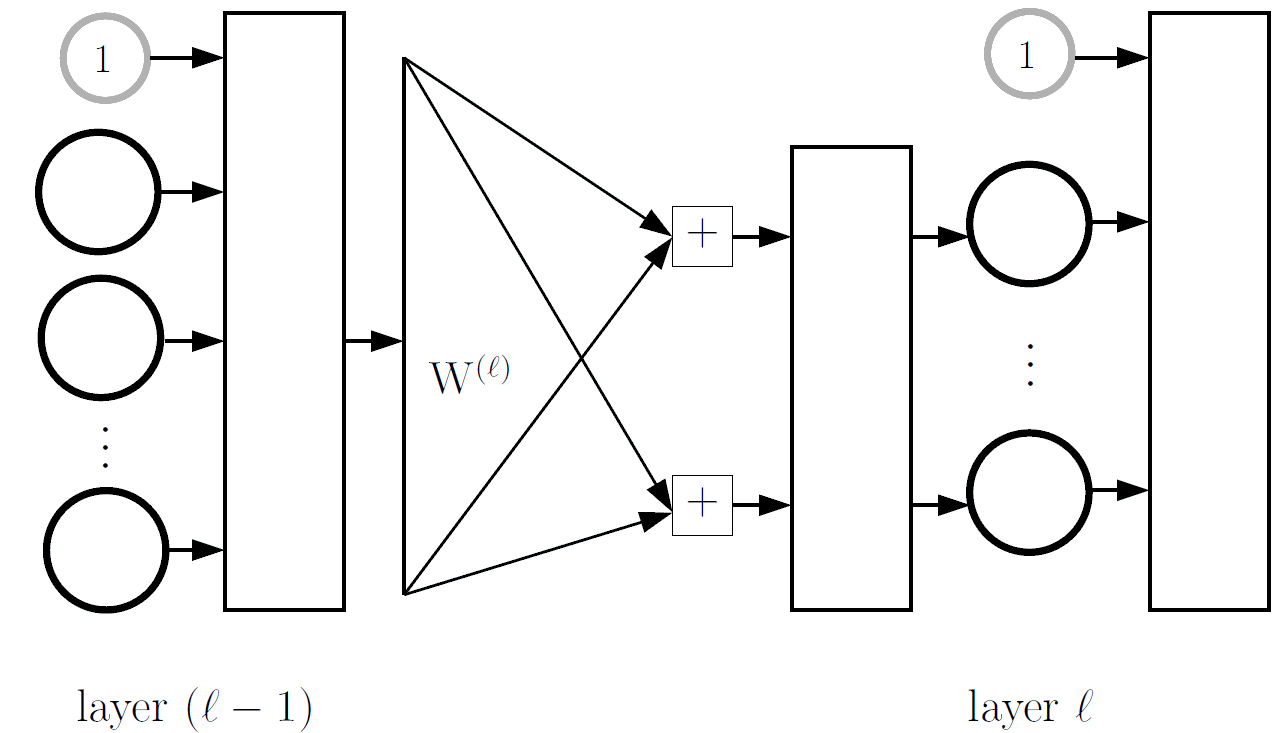
\includegraphics[width=0.8\linewidth]{images/vectorized_backprop.png}
        \caption{Vectorized data flow from the activations of the previous layer ($a^{[l-1]}$) to the current layer ($a^{[l]}$).}
    \end{figure}
\end{frame}